\subsection{Explicación formal del problema}

El problema dado se puede modelar como un grafo (no dirigido) en el cual cada vertice es un planeta y las aristas representan las rutas entre los mismos, estas tienen pesos asignados los cuales representan la cantidad de litros que requieren para ser recorridas. Como se aclara que se puede llegar de un planeta a cualquier otro, podemos asumir que el grafo es conexo.

El objetivo es, a partir de un nodo 0, visitar todos los demas gastando la menor cantidad de litros posible. Esta idea de visitar todos los vertices del grafo y al mismo tiempo gastar la menor cantidad de litros se puede traducir a buscar un subgrafo de ciertas particularidades, entre otras cosas que comparta los mismos nodos que el grafo original pero sacando las aristas que no valgan la pena recorrer porque podemos atravesar otras menos costosas, pero de esto hablaremos en mas detalle en la siguiente parte del informe, por ahora veamos algunos ejemplos de soluciones validas e invalidas.

Dado el el grafo de la figura (\ref{fig:ej-2.1}), el nodo 0 es el inicial y debemos visitar todos los demas.

\begin{figure}[H]
\centering
\begin{minipage}[b]{0.4\textwidth}
\centering
%
\begin{tikzpicture}[>=stealth',shorten >=1pt,auto,node distance=2.8cm,
                    semithick]
  \tikzstyle{every state}=[fill=red,draw=none,text=white]

  \node[state, fill = blue]         (A)                    {$0$};
  \node[state]         (B) [above right of=A] {$1$};
  \node[state]         (D) [below right of=A] {$2$};
  \node[state]         (C) [below right of=B] {$3$};
  \node[state]         (E) [below of=D]       {$4$};

  \path (A) edge              node {10} (B)
        		edge[bend right]	 node {8} (E)            
        (B) edge              node {5} (C)
        (C) edge              node {4} (D)
            edge [bend left]  node {1} (E)
            edge              node {1} (A);
\end{tikzpicture}
\caption{\footnotesize{Ejemplo de una instancia posible del problema.}} 
\end{minipage}
\label{fig:ej-2.1}
%
\hfill
%
\begin{minipage}[b]{0.4\textwidth}
\centering
\begin{tikzpicture}[>=stealth',shorten >=1pt,auto,node distance=2.8cm,
                    semithick]
  \tikzstyle{every state}=[fill=red,draw=none,text=white]

  \node[state, fill = blue]         (A)                    {$0$};
  \node[state]         (B) [above right of=A] {$1$};
  \node[state]         (D) [below right of=A] {$2$};
  \node[state]         (C) [below right of=B] {$3$};
  \node[state]         (E) [below of=D]       {$4$};

  \path (B) edge              node {5} (C)
        (C) edge              node {4} (D)
            edge [bend left]  node {1} (E)
            edge              node {1} (A);
\end{tikzpicture}
\caption{\footnotesize{El recorrido representado es óptimo. }}
\end{minipage}
\end{figure}


\begin{figure}[H]
\centering
\begin{minipage}[b]{0.4\textwidth}
\centering
%
\begin{tikzpicture}[>=stealth',shorten >=1pt,auto,node distance=2.8cm,
                    semithick]
  \tikzstyle{every state}=[fill=red,draw=none,text=white]

  \node[state, fill = blue]         (A)                    {$0$};
  \node[state]         (B) [above right of=A] {$1$};
  \node[state]         (D) [below right of=A] {$2$};
  \node[state]         (C) [below right of=B] {$3$};
  \node[state]         (E) [below of=D]       {$4$};

  \path (B) edge              node {5} (C)
  			edge				  node {10}(A)
        (C) edge              node {4} (D)
            edge [bend left]  node {1} (E)
            edge              node {1} (A);
\end{tikzpicture}
\caption{\footnotesize{El recorrido representado no es óptimo. Si bien tiene todos los caminos mínimos también tiene uno de mas, el camino directo del vertice 0 al 1, este agrega un costo de 10 el cual es innecesario ya que por mas que no estuviera podiamos ir de todas maneras con costo 6 hasta ese planeta.}}
\end{minipage}
\hfill
\begin{minipage}[b]{0.4\textwidth}
\centering
%
\begin{tikzpicture}[>=stealth',shorten >=1pt,auto,node distance=2.8cm,
                    semithick]
  \tikzstyle{every state}=[fill=red,draw=none,text=white]

  \node[state, fill = blue]         (A)                    {$0$};
  \node[state]         (B) [above right of=A] {$1$};
  \node[state]         (D) [below right of=A] {$2$};
  \node[state]         (C) [below right of=B] {$3$};
  \node[state]         (E) [below of=D]       {$4$};
%
  \path (A) edge              node {10} (B)
        		edge[bend right]  node {8} (E)            
        (B) edge              node {5} (C)
        (C) edge              node {4} (D);
%
\end{tikzpicture}
\caption{\footnotesize{El recorrido representado por el grafo no es una solución ya que hubiera sido mas económico reemplazar el trayecto de 0 a 3 por un camino directo de costo 1, o reemplazar el costo de 0 a 1 por un camino indirecto de costo 2 en vez de el camino directo de costo 8. }}
\end{minipage}
\end{figure}

\subsection{Explicación de la solución}

Como ya dijimos el problema se puede entender como un grafo, en el cual debemos a partir del nodo 0 visitar todos los demás. Este recorrido solución no va a tener ciclos ya que eso implicaria que pasamos dos veces por el mismo planeta agregando un costo innecesario y va a ser conexo ya que sino significaría que hay planetas que no podemos visitar, sabiendo esto y que queremos que el recorrido sea de costo mínimo se deduce que lo que estamos buscando es equivalente al cálculo de un árbol generador mínimo. Para realizar esto decidimos utilizar uno de los algoritmos vistos en la teórica. En los siguientes párrafos hablaremos de como realizamos su implementación, porqué es correcto y cual es su complejidad.

\subsubsection{Explicación del código}

Para este ejercicio el código es un poco mas extenso que en los demás debido a que se tuvo que crear un heap que cumpla ciertas particularidades. Si bien en gran parte es un heap binario clásico se diferencia en que tiene un vector extra llamado $pos$ que almacena la posición de cada nodo en el heap, esto es para asegurar un costo de $O(log(n))$ en ciertas operaciones. Los vertices del heap, llamados $vertex$ estan formados por dos $integers$, primero $key$ el cual es el nombre que le asignamos al nodo y segundo $value$ que representará la menor distancia encontrada hasta el momento desde su candidato a padre hasta dicho vértice.

Conociendo las operaciones usuales de un heap y habiendo resaltado las caracteristicas distintivas de nuestra implementación veamos ahora como realizamos la función $prim$, esta toma un heap de $n$ vértices, el cual esta inicializado con el $value$ del nodo $0$ en $0$ y todos los demás con $\infty$, las $keys$ numeran todos los nodos de $0$ a $n-1$. Estos valores obligan al heap a tener como raiz al nodo 0 (ya que se ordena por value de menor a mayor y el 0 es el mas pequeño). Como segunda variable de entrada esta la lista de adyacencia del grafo.

El programa devuelve un vector $parent$ de tamaño $n$ el cual indica que en el AGM resultante el nodo i tiene como padre al nodo $parent[i].first$ y para llegar a el desde su padre se gastan $parent[i].second$ litros.

\subsubsection{Pseudocódigo}

\begin{algorithm}[H]
  \begin{algorithmic}[1]
  \caption{Pseudocódigo de Prim}
  \label{algo:2-1}
    \Procedure{prim}{\texttt{MinHeap} $heap$, \texttt{Vector<VerticesAdyacentes>} $adj\_list$} $\rightarrow$ \texttt{Vector<int,int>}
    	\State \texttt{Vector<int,int>} $parent(heap.Size(), <0,0>)$
    	\Comment $O(n)$
    	\While{$ heap.Size() > 0 $}
    		\Comment $O(n)$ veces
    		\State \texttt{Vertex} $min\_vertex \gets heap.Pop()$
    		\Comment $O(log(n))$
    		\State \texttt{int} $ u \gets min\_vertex.key$
    		\Comment $O(1)$
    		\For{$ vertex\_and\_weight \in adj\_list[u] $}
    		\Comment $O(d(u))$ veces
	    		\State \texttt{int} $ v \gets vertex\_and\_weight.first$
	    		\Comment $O(1)$    			
	    		\State \texttt{int} $ weight \gets vertex\_and\_weight.second$
	    		\Comment $O(1)$    			
    			\If{$ heap.At(v) \land weight < heap.Value(v) $}
    			\Comment $O(1)$
    				\State $parent[v].first \gets u$
    				\Comment $O(1)$
    				\State $parent[v].second \gets weight$
    				\Comment $O(1)$
    				\State $heap.DecValue(v, weight)$
    				\Comment $O(log(n))$
    			\EndIf
    		\EndFor
    	\EndWhile
    	\State \texttt{return} $parent$
		\EndProcedure
	\end{algorithmic}
\end{algorithm}

Intentemos entender que es lo que hace este algoritmo y luego veremos por qué es correcto y óptimo.

Primero se construye $parent$ el vector de tuplas inicializado en pares de dos ceros. 

Luego se comienza a iterar, en cada iteración se sacará el vertice de menor $value$ del heap, estos ya no serán mas actualizados en el vector $parent$ por lo que su posición en el árbol quedá determinada en ese momento. Luego se ve por cada uno de sus vertices adyacentes si actualizar $parent$ o no. Como se observa en la guarda del $if$ esto sucederá si el vector adyacente esta aún en el heap y si su distancia al último nodo que se extrajo de la cola es menor que el valor que tiene actualmente en el heap. En ese caso se actualizará su valor en el heap y se guardara su nuevo padre y su nuevo peso en $parent$.

\subsubsection{Correctitud y Optimalidad}

Veamos porque el algoritmo de Prim es correcto, o sea, dado un grafo $G$ conexo y ponderado nos asegura conseguir un árbol generador mínimo.

Primero veamos que el resultado describe realmente un arbol generador. Como el grafo es conexo y en el heap todos los nodos arrancan con $value = \infty$ eventualmente todos los nodos caen al menos una vez dentro del if teniendo agregando asi al vector de salida un padre y la distancia a la que estan de el. El resultado final por lo tanto nos da un árbol debido a que cada nodo tiene un único padre y es generador de G por haber sido formado a partir de sus propios nodos y aristas.

Veamos ahora porque este grafo, A, es mínimo. Como la cantidad de árboles generadores de un grafo es finita existe alguno que es el mínimo, llamemoslo $A'$. Si A e igual a A' entonces es un AGM. Si no lo es, sea $e$ la primera arista agregada durante la construcción de A, que no está en A' y sea V el conjunto de nodos conectados por las aristas agregadas antes que e. Entonces un extremo de e está en V y el otro no. Ya que A' es el árbol generador mínimo de G hay un camino en A' que uno los dos extremos. Mientras que uno se mueve por el camino, se debe encontrar una arista f uniendo un nodo de en V a uno que no está en V. En la iteracion que e se agrega a A, f también se podría haber agregado y se hubiese agregado en vez de e si su peso fuera menor que el de e. Ya que f no se agrego se concluye que P(f) $\geq$ P(e).

Sea A'' el grafo obtenido al remover f y agregar e a A'. Es fácil mostrar que A'' es conexo y tiene la misma cantidad de aristas que A', y el peso total de sus aristas no es mayor que el de A', entonces también es un AGM de G y contiene a e y todas las aristas agregadas anteriormente durante la construcción de V. Si se repiten los pasos mencionados anteriormente, eventualmente se obentrá el árbol generador mínimo de G que es igual a A.

Esto demuestra que A es el AGM de G.


\subsection{Complejidad del algoritmo}

Dado un G conexo y ponderado, nuestro algoritmo tendrá una complejidad de $\theta(m.log(n))$ para el peor caso, está podra ser mejorada para algunas instancias consiguiendo $\theta(m + n.log(n))$.

Analicemos de donde salen dichas afirmaciones. La función main esta compuesta por la primer parte donde  genera un vector de adyacencia, primero inicializado en valores nulos $\theta(n)$ y luego llenado con los datos de entrada $\theta(m)$.

Luego se crea un vector $v\_inicial$ el cual será el heap que recibirá de entrada la función $prim$ este se llena con n nodos, el primero inicializado en $0$ y los demás con $value$ infinito y un $key$ distintivo entre $1$ y $n-1$. Esto cuesta $\theta(n)$. Para convertirlo luego en un heap se utiliza $MinHeap$ que cuesta $O(n.log(n))$ por utilizar n veces a la función $MinHeapify$ que es $O(log(n))$.

Una vez hecho esto se llama a prim, viendo el pseudocódigo se puede ver que realizamos por cada vértice adyacente de cada nodo una operación que cuesta a lo sumo $O(log(n))$ si caemos dentro del if, agregado a lo que seguro que hacemos con cada nodo que cuesta $O(log(n))$ ($pop()$ mas otras operaciones de costo constante).

La complejidad resultante de prim si caemos dentro de todos los if (peor caso) será:

	$$O( \sum_{i=0}^{n-1}d(v_{i}).log(n) + n.log(n) ) = $$
	$$O( (\sum_{i=0}^{n-1}d(v_{i}) + n).log(n) ) = $$
	$$O( (2m + n).log(n) ) = O( 2m.log(n) ) = O(m.log(n))$$ 

Notar que podemos prescindir de n en la suma 2m+n ya que el grafo es conexo y por lo tanto n será menor a 2m.

Finalmente se calcula el peso del árbol con una complejidad temporal de $O(n)$ a partir del vector de salida de $prim$ y se imprime a la salida.

Sumando todo lo dicho se ve que nada supera la complejidad de $prim$ por lo que el costo final quedá limitado por este en $O(m.log(n))$

Si solo cayeramos n veces en el if (mejor caso) entonces la complejidad de prim será
	$$O( \sum_{i=0}^{n-1}d(v_{i}) - n + n.log(n) + n.log(n) ) = $$
	$$O( \sum_{i=0}^{n-1}d(v_{i}) - n + 2.n.log(n) ) = $$
	$$O( 2m - n + n.log(n) ) = O( m + n.(log(n)-1) ) $$

\subsection{Performance del algoritmo}


\begin{figure}[H]
 \centering
	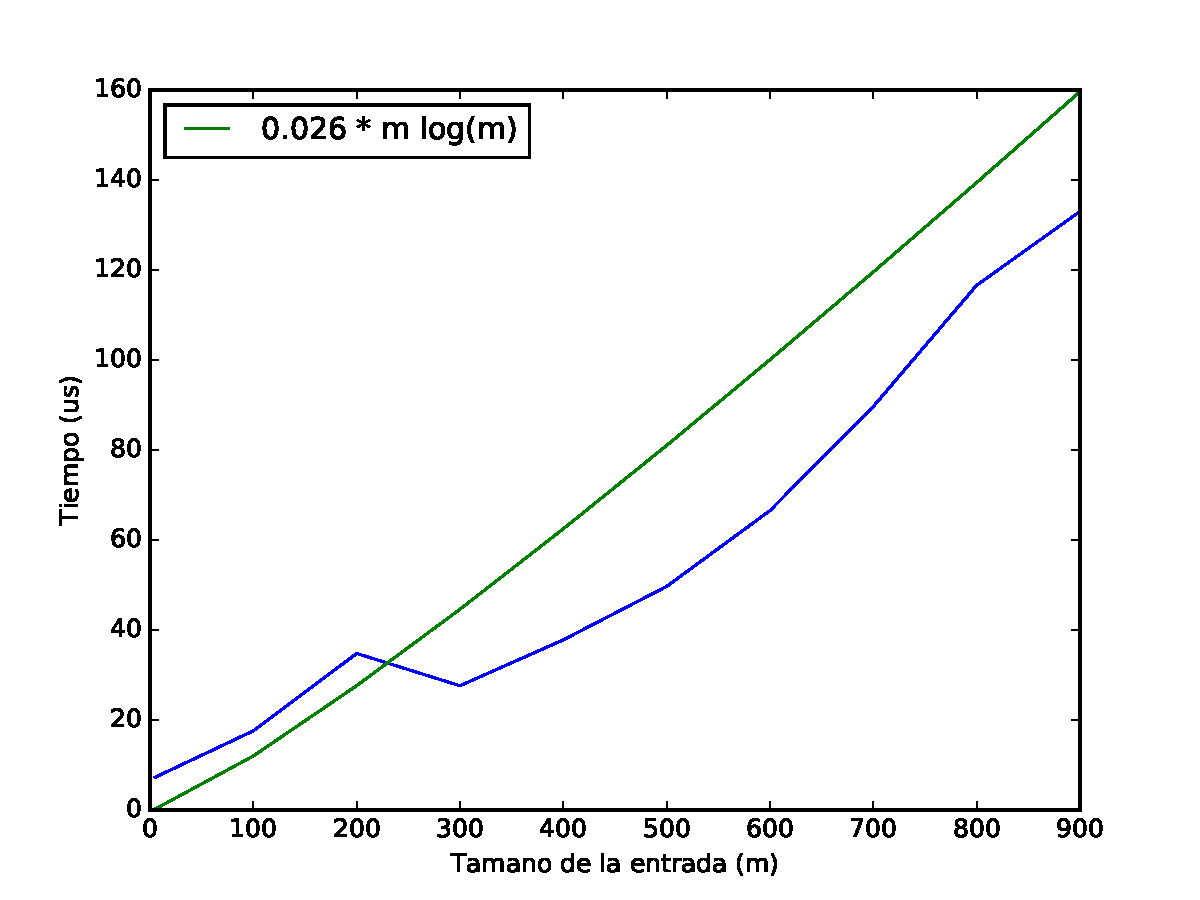
\includegraphics[width=0.8\textwidth]{img/exp/problema2-promedio.pdf}
	\caption{\footnotesize Tiempo que toma el algoritmo en $\mu$s para una entrada de tamaño $m$. $n$ al azar.}
	\label{fig:problema2-promedio}
\end{figure}

\begin{figure}[H]
 \centering
	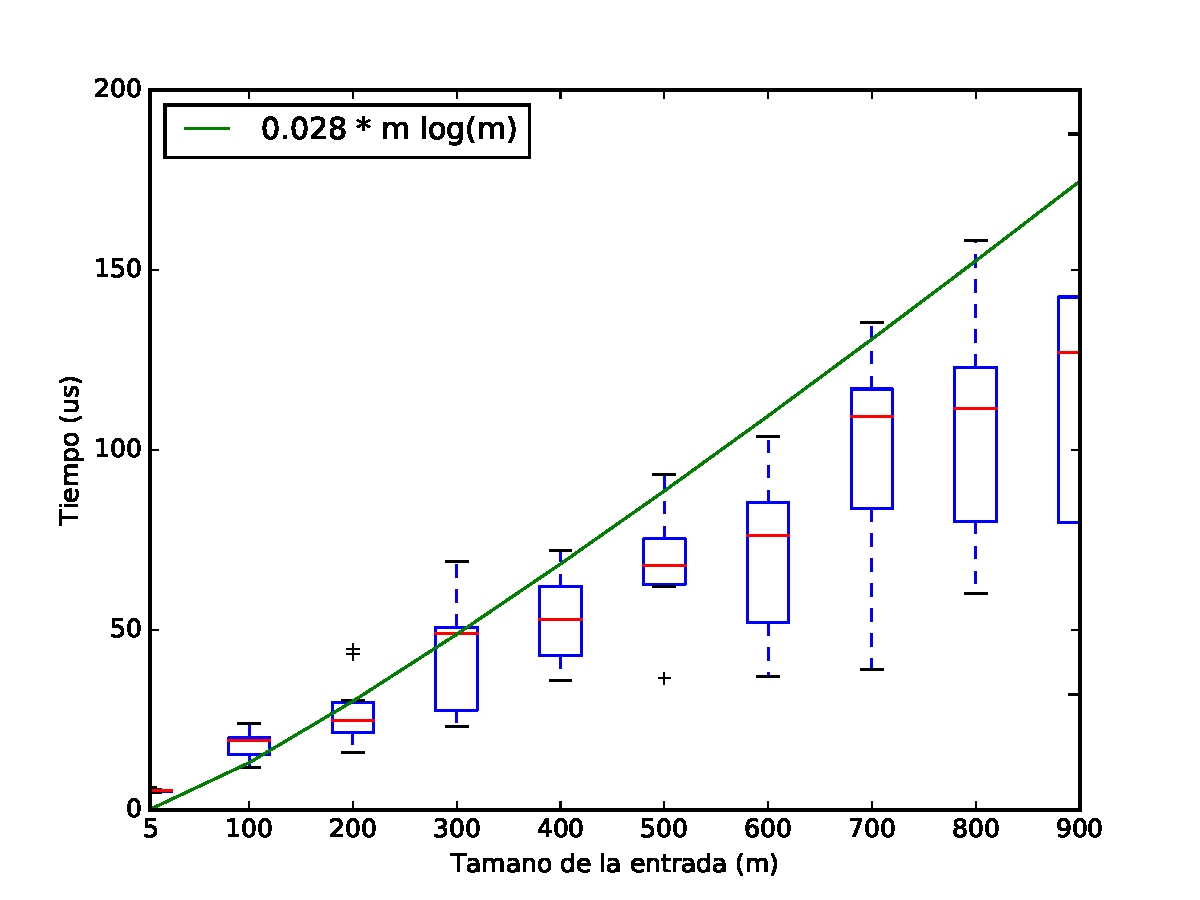
\includegraphics[width=0.8\textwidth]{img/exp/problema2-promedio2.pdf}
  \caption{\footnotesize Tiempo que toma el algoritmo en $\mu$s para una entrada de tamaño $m$. $n$ al azar. Se indican los valores del primer al tercer cuartil con un rectángulo azul y la mediana con una linea roja. El máximo y minimo se indican con lineas negras arriba y abajo del rectángulo.}
	\label{fig:problema2-promedio2}
\end{figure}

\begin{figure}[H]
 \centering
	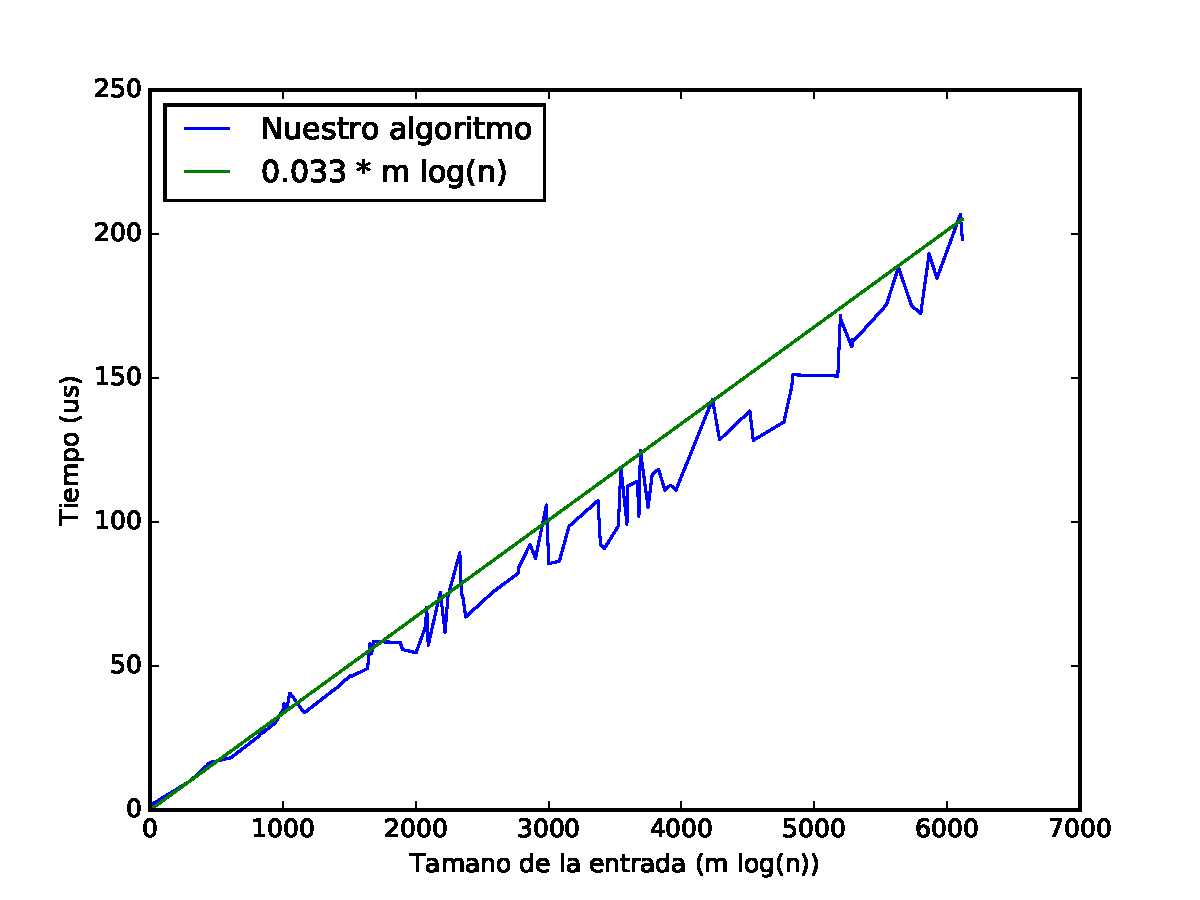
\includegraphics[width=0.8\textwidth]{img/exp/problema2-posta.pdf}
	\caption{\footnotesize Tiempo que toma el algoritmo en $\mu$s para una entrada de tamaño $m \log n$.}
	\label{fig:problema2-posta}
\end{figure}


\subsubsection{M\'etodo de experimentación}

